
  

% --------------------------------------------------------------
% This is all preamble stuff that you don't have to worry about.
% Head down to where it says "Start here"
% --------------------------------------------------------------

\documentclass[10pt]{article}

\usepackage{bera}
%\renewcommand{\familydefault}{\rmfamily}

\usepackage{graphicx,url}
\usepackage{proof}
\usepackage{framed}
\usepackage{etaremune}
\usepackage{tcolorbox}
\usepackage{fancyvrb}
\usepackage{graphics}
\usepackage{minibox}
\usepackage{amssymb}
\usepackage[margin=1in]{geometry}
\usepackage{amsmath,amsthm,amssymb,amsfonts}
\usepackage{paralist}
\thispagestyle{empty}

% 1. To get version suitable for students to populate,
%    remove the contents of the \ignoreSoln{..body..}
%
% 2. To get a version suitable for generating PDF 
%    without solutions, remove the #1 below
%
% 3. To generate solutions, keep the #1 below
%
% 4. Assigned grader fills \ignoreSoln{..body..}
%    and also provides his/her feedback to student
%    and policy followed for point deduction
%    So design policy before grading begins.

\newcommand{\ignoreSoln}[1]{#1}   
%\newcommand{\ignoreModel}[1]{#1} 


\newcommand{\bigset}[2]{\big\{\;#1\;:\;#2\;\big\}}
\newcommand{\N}{\mathbb{N}}
\newcommand{\Z}{\mathbb{Z}}
\newcommand{\R}{\mathbb{R}}
\newcommand{\Np}{\mathbb{N^{+}}}

\newenvironment{theorem}[2][Theorem]{\begin{trivlist}
\item[\hskip \labelsep {\bfseries #1}\hskip \labelsep {\bfseries #2.}]}{\end{trivlist}}
\newenvironment{lemma}[2][Lemma]{\begin{trivlist}
\item[\hskip \labelsep {\bfseries #1}\hskip \labelsep {\bfseries #2.}]}{\end{trivlist}}
\newenvironment{exercise}[2][Exercise]{\begin{trivlist}
\item[\hskip \labelsep {\bfseries #1}\hskip \labelsep {\bfseries #2.}]}{\end{trivlist}}
\newenvironment{reflection}[2][Reflection]{\begin{trivlist}
\item[\hskip \labelsep {\bfseries #1}\hskip \labelsep {\bfseries #2.}]}{\end{trivlist}}
\newenvironment{proposition}[2][Proposition]{\begin{trivlist}
\item[\hskip \labelsep {\bfseries #1}\hskip \labelsep {\bfseries #2.}]}{\end{trivlist}}
\newenvironment{corollary}[2][Corollary]{\begin{trivlist}
\item[\hskip \labelsep {\bfseries #1}\hskip \labelsep {\bfseries #2.}]}{\end{trivlist}}

\DeclareMathSizes{14}{14}{14}{14}

\begin{document}

% --------------------------------------------------------------
%                         Start here
% --------------------------------------------------------------

%\renewcommand{\qedsymbol}{\filledbox}


\begin{center}
\begin{large}
  CS 6110, Spring 2022, Assignment 1  \\
  Given 1/13/22 -- Due 1/20/22 by 11:59 pm on Canvas
  \ \\
%  \ \\  
      {  {\Large\bf NAME: Tripti Agarwal} \hfill {\Large\bf UNID: u1319433}\hspace{4cm} }
\end{large}
\end{center}
 

\date{}



%



%- 1 ----------------------------------------------------------------

\begin{enumerate}
\item \textbf{Reading from Bradley's book} 
\newlength{\minpagw}
\settowidth{\minpagw}{\hspace{40em}}

\begin{minipage}{\minpagw}
  \fbox{%
    \parbox{\linewidth}{%
      \begin{enumerate}
          \item \textbf{Satisfiability:} A formula $F$ is satisfiable iff there exists an interpretation $I$ such that $I \models F$
          \item \textbf{Validity:} A formula $F$ is valid iff for all interpretations $I$, $I \models F$. A formula is valid if all the values for the final value of the truth table is 1. To prove a formula is valid using semantics, we prove it by contradiction. Rules for semantic proving are:
          \begin{itemize}
              \item $I \models \lnot  F$, deduce $I \nvDash F$; and from $I \nvDash  \lnot  F$, deduce $I \models F$
              \item  from $I \models F \wedge G$, deduce both $I \models F$ and $I \models G$; and from $I \nvDash F \wedge G$, deduce $I \nvDash F$ or $I \nvDash  G$
              \item  from $I \models F \veeG$, deduce $I \models F$ or $I \models G$; and from $I \nvDash F \vee G$, deduce both $I \nvDash F$ and $I \nvDash G$
              \item $I \models F \rightarrow G$, deduce $I \nvDash F$ or $I \models G$; and from $I \nvDash F \rightarrow G$, deduce both $I \models F$ and $I \nvDash G$.
              \item  from $I \models F \leftrightarrow G$, deduce $I \models F \wedge G$ or $I \nvDash F \vee G$; and from $I \nvDash F \leftrightarrow G$, deduce $I \models F \wedge \lnot  G$ or $I \models \lnot  F \wedge G$
              \item $I \implies F$ and $I \nvDash F$ then $I \models \bot$
          \end{itemize}
          \item \textbf{Equivalence:} Two formulae $F_1$ and $F_2$ are equivalent if they evaluate to the same truth value under all interpretations $I$. That is, for all interpretations $I$, $I \models F_1$ iff $I \models F_2$. In truth table all the final values should be 1. In semantic logic we prove two formulae are equivalence using the method of contradiction.
          \item \textbf{Normal Form:} A normal form of formulae is a syntactic restriction such that for every formula of the logic, there is an equivalent formula in the normal form.
          \begin{itemize}
              \item \textbf{Negation normal form (NNF)} requires that $\lnot$, $\wedge$, and $\vee$ be the only connectives and that negations appear only in literals. When implementing the transformation, the equivalences should be applied left-to-right.
              \item A formula is in \textbf{disjunctive normal form (DNF)} if it is a disjunction of conjunctions of literals. $\vee_i \wedge_j l_{i,j}$ for literals $l_{i,j}$   
              \item The dual of DNF is \textbf{conjunctive normal form (CNF}). A formula in CNF is a conjunction of disjunctions of literals. $\wedge_i \vee_j l_{i,j}$ for literals $l_{i,j}$ 
              \end{itemize}
      \item \textbf{ Decision Procedures for Satisfiability}
      \begin{itemize}
          \item Simple Decision Procedures: Using truth tables
          \item Coversion of equisat problems to CNF
      \end{itemize}
      \end{enumerate}
    }%
  }%
\end{minipage}

\clearpage

%- 2 ----------------------------------------------------------------

\item \textbf{Understanding Equisat Versus Equivalence}. \begin{itemize}
  \item A code cell

    \begin{Verbatim}[frame=single]
EquiSat = '''
Var_Order : a,b,c,p,z
fGiven = (c|(a&b))
fTseitin = z &(~p|a) & (~p|b) & (~a|~b|p) &(~z|p|c) & (~p|z) & (~c|z)
Main_Exp : fTseitin -> fGiven 
\end{Verbatim}


  
  

\item 

\begin{Verbatim}[frame=single]
buildBDDmain(EquiSat.splitlines())
import graphviz
from IPython.display import Image
import pydot
graphs = pydot.graph\_from\_dot\_file(final\_dot\_file+".dot")
graph = graphs[0]
graph.write\_png(final\_dot\_file+'.png')
from IPython.display import ImageImage(final\_dot\_file+'.png',
width=300)
\end{Verbatim}

\end{itemize}
  
  Now answer these questions:
  
  \begin{enumerate}
  \item Which case (\verb|->| or \verb|<-|) gave you a ``1'' node and why?

  \item[] \framebox{fTseitin $\rightarrow$ fGiven
  }
  \begin{Verbatim}[frame=single]
  This is because the two implications are not equivalent. For the 
  formulas when fTseitin -> fGiven, those CNF formula results in
  formulae that is satisfiable to the given formula, whereas for the
  implication other way i.e. fGiven -> fTseitin is not. 
  Hence, fGiven <-> fTseitin is equisat and not equivalent.
  
  \end{Verbatim}

  \item Within the case
    where you did  get a ``0'' node,
    insert that BDD which has 0 here.
  \begin{Verbatim}[frame=single]
EquiSat = '''
Var_Order : a,b,c,p,z
fGiven = (c|(a&b))
fTseitin = z &(~p|a) & (~p|b) & (~a|~b|p) & (~z|p|c) & (~p|z) & (~c|z)
Main_Exp :  fGiven -> fTseitin # Also <-> 
\end{Verbatim}
  \item
    for all the paths to the ``0'' node,
    explain why that path exists (this is where equisat differed from equivalence).
    Write out your answer in neat bulletted steps per path.
  
\newlength{\minpagw}
\settowidth{\minpagw}{\hspace{40em}}

\begin{minipage}{\minpagw}
  \fbox{%
    \parbox{\linewidth}{%
\begin{itemize}
    \item\textbf{ [1,1,c,0,z]} : where c and z can have either 0 or 1. This is because when p $\rightarrow$ a.b is satisfiable but a.b $\rightarrow$ p is not. As the formula is equisat and not equivalent. 
    \item \textbf{[1,1,c,1,0]} : where c can have either 0 or 1. This is because when p $\rightarrow$ a.b is satisfiable but a.b $\rightarrow$ p is not. 
    \item \textbf{[1,0,1,0,0]} : This is because when  z $\rightarrow$ p$\vee$c is satisfiable but p$\vee$c $\rightarrow$ z is not.
    \item \textbf{[1,0,1,1,z]} : where z can have either 0 or 1. This is because when  z $\rightarrow$ p$\vee$cis satisfiable but p$\vee$c $\rightarrow$ z is not, when z = 0.
    \item \textbf{[0,b,1,1,z]} : where b and z can have either 0 or 1.  This is because when  z $\rightarrow$ p$\vee$c is satisfiable but p$\vee$c $\rightarrow$ z is not, when z = 0. 
    \item \textbf{[0,b,1,0,0]} : where b can have either 0 or 1. This is because when  z $\rightarrow$ p$\vee$c is satisfiable but p$\vee$c $\rightarrow$ z is not.
\end{itemize}
    }%
  }%
\end{minipage}

\clearpage

  \end{enumerate}

  \clearpage
  
%- 3 ----------------------------------------------------------------
 
\item \textbf{Buggy bubble sort}\\
  \begin{itemize}
      \item 
  \textbf{Commands and flags used}\\
  \framebox{spin -a bubblesort.pml}\\
 \framebox{gcc -DMEMLIM=1024 -O2 -w -o pan pan.c} \\
 \framebox{./pan}
 \item \textbf{Run Results}
  \begin{Verbatim}[frame=single]
pan:1: assertion violated 0 (at depth 11)
pan: wrote bubblesort.pml.trail
(Spin Version 6.4.9 -- 17 December 2018)
Warning: Search not completed
	+ Partial Order Reduction
Full statespace search for:
	never claim         	- (none specified)
	assertion violations	+
	acceptance   cycles 	- (not selected)
	invalid end states	+
State-vector 20 byte, depth reached 20, errors: 1
       44 states, stored
        7 states, matched
       51 transitions (= stored+matched)
        0 atomic steps
hash conflicts:         0 (resolved)
Stats on memory usage (in Megabytes):
    0.002	equivalent memory usage for states 
    (stored*(State-vector + overhead))
    0.287	actual memory usage for states
  128.000	memory used for hash table (-w24)
    0.534	memory used for DFS stack (-m10000)
  128.730	total actual memory usage
pan: elapsed time 0 seconds

  \end{Verbatim}
  \item \textbf{Error Tracing:} \framebox{spin -p -t bubblesort.pml}\\
  \begin{Verbatim}[frame=single]
  1:	proc  0 (bubsort:1) bubblesort.pml:16 (state 2)
  [a[1] = 1]
  2:	proc  0 (bubsort:1) bubblesort.pml:16 (state 3)
  [a[2] = 1]
  3:	proc  0 (bubsort:1) bubblesort.pml:16 (state 1)
  [goto :b0]
  3:	proc  0 (bubsort:1) bubblesort.pml:18 (state 9)
  [t = a[1]]
  3:	proc  0 (bubsort:1) bubblesort.pml:18 (state 10)
  [j = (1+1)]
  4:	proc  0 (bubsort:1) bubblesort.pml:22 (state 13)
  [((j<=(5-1)))]
  5:	proc  0 (bubsort:1) bubblesort.pml:25 (state 18)
  [((a[(j-1)]<=a[j]))]
  5:	proc  0 (bubsort:1) bubblesort.pml:27 (state 21)
  [j = (j+1)]
  6:	proc  0 (bubsort:1) bubblesort.pml:22 (state 13)
  [((j<=(5-1)))]
  7:	proc  0 (bubsort:1) bubblesort.pml:24 (state 14)
  [((a[(j-1)]>a[j]))]
  7:	proc  0 (bubsort:1) bubblesort.pml:24 (state 15)
  [t = a[(j-1)]]
  7:	proc  0 (bubsort:1) bubblesort.pml:24 (state 16)
  [a[(j-1)] = a[j]]
  7:	proc  0 (bubsort:1) bubblesort.pml:24 (state 17)
  [a[j] = t]
  7:	proc  0 (bubsort:1) bubblesort.pml:27 (state 21)
  [j = (j+1)]
  8:	proc  0 (bubsort:1) bubblesort.pml:22 (state 13)
  [((j<=(5-1)))]
  9:	proc  0 (bubsort:1) bubblesort.pml:24 (state 14)
  [((a[(j-1)]>a[j]))]
  9:	proc  0 (bubsort:1) bubblesort.pml:24 (state 15)
  [t = a[(j-1)]]
  9:	proc  0 (bubsort:1) bubblesort.pml:24 (state 16)
  [a[(j-1)] = a[j]]
  9:	proc  0 (bubsort:1) bubblesort.pml:24 (state 17)
  [a[j] = t]
  9:	proc  0 (bubsort:1) bubblesort.pml:27 (state 21)
  [j = (j+1)]
 10:	proc  0 (bubsort:1) bubblesort.pml:21 (state 11)
 [((j>(5-1)))]
 11:	proc  0 (bubsort:1) bubblesort.pml:42 (state 42)
 [((t==a[1]))]
 11:	proc  0 (bubsort:1) bubblesort.pml:45 (state 47)
 [t = 1]
 12:	proc  0 (bubsort:1) bubblesort.pml:49 (state 52)
 [((a[t]>a[(t+1)]))]
spin: bubblesort.pml:49, Error: assertion violated
spin: text of failed assertion: assert(0)
 12:	proc  0 (bubsort:1) bubblesort.pml:49 (state 53)
 [assert(0)]
spin: trail ends after 12 steps
#processes: 1
 12:	proc  0 (bubsort:1) bubblesort.pml:46 (state 54)
1 process created

  \end{Verbatim}
  \item \textbf{Fully explain all uses of nondeterminism in this Promela model.}\\
  \minibox[frame]{In the above program, we obtain an automata, and for any given input from one \\
  state to another there is a single output. Hence the automata does not have determinism.}
   
  \item \textbf{Fully explain also the use  of  data-abstraction  (i.e.,  we  got  away  with  using  “0”  and  “1”  in  sorting;  is  that representative-enough?)}\\
  \minibox[frame]{In the provided code, the elements of type bit is used i.e. each element in the array 'a'\\ is of type bit. Since the code is able to sort the elements using bit elements hence we\\ can get away for any number by just representing them using bits. }
  \item \textbf{Write a good para arguing that (modulo modeling-errors which are assumed not to be there) this model-checking ended-up verifying the sorting for the size you considered.  Can you extend your argument to say that this verification is good for arrays of any size?}\\
  \minibox[frame]{In general, to prove any sorting array, we need to have minimum of 3 elements to prove\\ it is correct. This is because, if we have only 1 element, there is nothing to sort and we\\ cannot prove that the model for sorting is correct or not. Let say we use an array of size\\ 2, probably this program can sort, but we can write another program that can do sorting \\for 2 elements but will end up not sorting correctly for array of size more than 2. \\Finally, if we choose the array of size 3, we apply the same bubble sort.\\ We observe that the program is able to produce the same error as with size 5. \\Hence, this verification is good enough to check for arrays of any size.}
  \end{itemize}


    \clearpage
%- 4 ----------------------------------------------------------------
  
  \item \textbf{Never Automata for Dinning Philospher}
    %
    Run this example under SPIN, and produce a violation trace showing that
    the never automaton ``accepts.'' This reveals a liveness violation.
    \begin{figure}[!h]
        \centering
        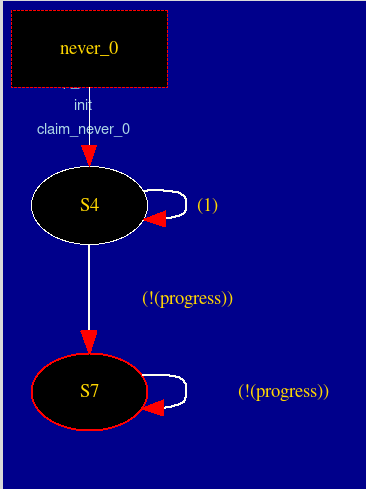
\includegraphics[width=0.5\textwidth]{never_phill.png}
        \caption{Never Automaton "accepts". It can be seen the figure that the trace enters the accept state (S7) at !progress and then it keeps looping in the same state. This is called weak fairness and is liveness violation as SPIN is looking for accepting cycles in the never claim. This is because !progress is a bad behaviour and we claim that our model does not have it. A never claim here is basically looking for negative behaviour, and this happens only when positive behaviour is negated. We can also see the never claim never terminates, showing that the model is incorrect. }
        \label{fig:my_label}
    \end{figure}
    
\end{enumerate}

    \clearpage
    
\subsection*{Diagramming, and Running SPIN on a terminal}

You must attempt to draw message-sequence charts on a notepad or ipad to debug effectively.
Please submit these with the assignment.
The URL \url{http://spinroot.com/spin/Man/Spin.html} gives you info on SPIN's flags.
There is more documentation on the {\bf spinroot} page.

\begin{scriptsize}
\begin{verbatim}
spin -a yourfile.pml
gcc -DMEMLIM=1024 -O2 -DXUSAFE -DSAFETY -DNOCLAIM -w -o pan pan.c
./pan -m10000 
Pid: 66796
(Once the pan binary is generated),
GET pan HELP AS FOLLOWS:
[ganesh@thinmac Examples]$ ./pan --help
saw option --
Spin Version 6.4.5 -- 1 January 2016
Valid Options are:
	-a,-l,-f  -> are disabled by -DSAFETY
	-A  ignore assert() violations
	-b  consider it an error to exceed the depth-limit
	-cN stop at Nth error (defaults to -c1)
	-D  print state tables in dot-format and stop
	-d  print state tables and stop
	-e  create trails for all errors
	-E  ignore invalid end states
	-hN use different hash-seed N:0..499 (defaults to -h0)
	-hash generate a random hash-polynomial for -h0 (see also -rhash)
	      using a seed set with -RSn (default 12345)
	-i  search for shortest path to error
	-I  like -i, but approximate and faster
	-J  reverse eval order of nested unlesses
	-mN max depth N steps (default=10k)
	-n  no listing of unreached states
	-QN set time-limit on execution of N minutes
	-q  require empty chans in valid end states
	-r  read and execute trail - can add -v,-n,-PN,-g,-C
	-r trailfilename  read and execute trail in file
	-rN read and execute N-th error trail
	-C  read and execute trail - columnated output (can add -v,-n)
	-r -PN read and execute trail - restrict trail output to proc N
	-g  read and execute trail + msc gui support
	-S  silent replay: only user defined printfs show
	-RSn use randomization seed n
	-rhash use random hash-polynomial and randomly choose -p_rotateN, -p_permute, or p_reverse
	-T  create trail files in read-only mode
	-t_reverse  reverse order in which transitions are explored
	-tsuf replace .trail with .suf on trailfiles
	-V  print SPIN version number
	-v  verbose -- filenames in unreached state listing
	-wN hashtable of 2^N entries (defaults to -w24)
	-x  do not overwrite an existing trail file
	options -r, -C, -PN, -g, and -S can optionally be followed by
	a filename argument, as in '-r filename', naming the trailfile
        [ganesh@thinmac Examples]$
== One tries to catch bugs at the most shallow depth ==
== SPIN also has a BFS mode and also a depth minimization mode ==
[ganesh@thinmac Examples]$ ./pan -m10000  <== search depth 
=== LOOK AT HOW ERRORS ARE SUMMARIZED AND REPORTED ===
=== You MUST read these bugs and warnings carefully! ===
=== Also read the statistics carefully! ===
pan:1: invalid end state (at depth 20)
pan: wrote atomicphil.pml.trail
(Spin Version 6.4.5 -- 1 January 2016)
Warning: Search not completed
	+ Partial Order Reduction
Full statespace search for:
	never claim         	- (not selected)         
	assertion violations	+                        
	cycle checks       	- (disabled by -DSAFETY) 
	invalid end states	+                        
 
State-vector 108 byte, depth reached 23, errors: 1        <==
       12 states, stored
        2 states, matched
       14 transitions (= stored+matched)
        5 atomic steps
hash conflicts:         0 (resolved)
Stats on memory usage (in Megabytes):
    0.002	equivalent memory usage for states (stored*(State-vector + overhead))
    0.291	actual memory usage for states
  128.000	memory used for hash table (-w24)
    0.534	memory used for DFS stack (-m10000)
  128.730	total actual memory usage
== THIS IS ERROR-TRAIL SIMULATON BELOW - understand all these flags! ==
[ganesh@thinmac Examples]$ spin -p -r -s -c  -t atomicphil.pml <-- just an example
proc 0 = :init:
using statement merging
Starting phil with pid 1 <-- just an example showing what to expect, is below
proc 1 = phil
  1:	proc  0 (:init::1) atomicphil.pml:28 (state 1)	[(run phil(p0,v0,p2,v2))]
Starting phil with pid 2
proc 2 = phil
  2:	proc  0 (:init::1) atomicphil.pml:32 (state 2)	[(run phil(p1,v1,p0,v0))]
Starting phil with pid 3
proc 3 = phil
  3:	proc  0 (:init::1) atomicphil.pml:36 (state 3)	[(run phil(p2,v2,p1,v1))]
Starting fork with pid 4
proc 4 = fork
  4:	proc  0 (:init::1) atomicphil.pml:39 (state 4)	[(run fork(p0,v0))]
Starting fork with pid 5
proc 5 = fork
  5:	proc  0 (:init::1) atomicphil.pml:41 (state 5)	[(run fork(p1,v1))]
Starting fork with pid 6
proc 6 = fork
  6:	proc  0 (:init::1) atomicphil.pml:43 (state 6)	[(run fork(p2,v2))]
q\p   0   1   2   3   4   5   6
  5   .   .   .   lfp!0
  7:	proc  3 (phil:1) atomicphil.pml:4 (state 1)	[lfp!0]
  5   .   .   .   .   .   .   p?0
  8:	proc  6 (fork:1) atomicphil.pml:10 (state 1)	[p?0]
  3   .   .   .   rfp!0
  9:	proc  3 (phil:1) atomicphil.pml:4 (state 2)	[rfp!0]
  3   .   .   .   .   .   p?0
 10:	proc  5 (fork:1) atomicphil.pml:10 (state 1)	[p?0]
                  Eating 11:	proc  3 (phil:1) atomicphil.pml:4 (state 3)	[printf('Eating')]
  6   .   .   .   lfv!0
 12:	proc  3 (phil:1) atomicphil.pml:4 (state 4)	[lfv!0]
  6   .   .   .   .   .   .   v?0
 13:	proc  6 (fork:1) atomicphil.pml:11 (state 2)	[v?0]
  1   .   lfp!0
 14:	proc  1 (phil:1) atomicphil.pml:4 (state 1)	[lfp!0]
  1   .   .   .   .   p?0
 15:	proc  4 (fork:1) atomicphil.pml:10 (state 1)	[p?0]
  4   .   .   .   rfv!0
 16:	proc  3 (phil:1) atomicphil.pml:4 (state 5)	[rfv!0]
  4   .   .   .   .   .   v?0
 17:	proc  5 (fork:1) atomicphil.pml:11 (state 2)	[v?0]
  5   .   .   .   lfp!0
 18:	proc  3 (phil:1) atomicphil.pml:4 (state 1)	[lfp!0]
  5   .   .   .   .   .   .   p?0
 19:	proc  6 (fork:1) atomicphil.pml:10 (state 1)	[p?0]
  3   .   .   lfp!0
 20:	proc  2 (phil:1) atomicphil.pml:4 (state 1)	[lfp!0]
  3   .   .   .   .   .   p?0
 21:	proc  5 (fork:1) atomicphil.pml:10 (state 1)	[p?0]
spin: trail ends after 21 steps
-------------
final state:
-------------
#processes: 7
 21:	proc  6 (fork:1) atomicphil.pml:11 (state 2)
 21:	proc  5 (fork:1) atomicphil.pml:11 (state 2)
 21:	proc  4 (fork:1) atomicphil.pml:11 (state 2)
 21:	proc  3 (phil:1) atomicphil.pml:4 (state 2)
 21:	proc  2 (phil:1) atomicphil.pml:4 (state 2)
 21:	proc  1 (phil:1) atomicphil.pml:4 (state 2)
 21:	proc  0 (:init::1) atomicphil.pml:46 (state 8) <valid end state>
7 processes created
=== NOW FIND OUT WHY THE ABOVE IS DESCRIBING A DEADLOCK ===


=== Drawing a diagram will help                         ===
\end{verbatim}

\minibox[frame]
{In the dinning philospher's problem, from the above first thing we can observe is all three philosphers are waiting for the fork.\\
The following diagrams can help understand that:}
\begin{figure}
    \centering
    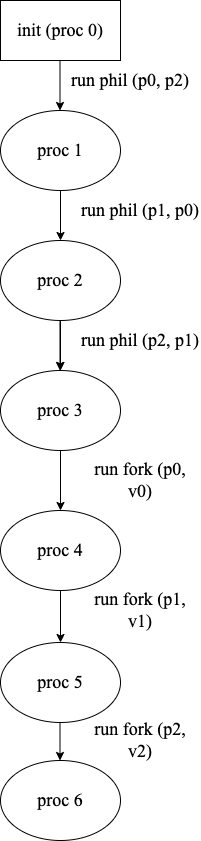
\includegraphics[width=0.2\textwidth]{StateDiag1.png}
    \caption{init automata}
    \label{fig:my_label}
\end{figure}
\begin{figure}
    \centering
    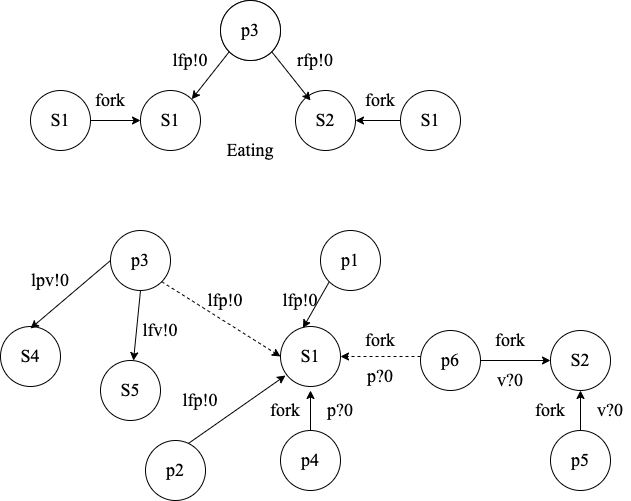
\includegraphics[width=\textwidth]{StateDiag2.png}
    \caption{Phil and fork automata for above output. We can see that p0, p1 and p2 are waiting for S1 ans none of the philospher is able to eat.}
    \label{fig:my_label}
\end{figure}
\end{scriptsize}
\end{document}


